\documentclass[11pt]{article}

\usepackage{color}
\usepackage{xcolor}
\usepackage{enumitem}
\usepackage{fancyhdr}
\usepackage{fancyvrb}
\usepackage{listings}
\usepackage{amsmath}
\usepackage{float}
\usepackage[T1]{fontenc}
\usepackage[utf8]{inputenc}
\usepackage{pmboxdraw}
\usepackage{graphicx}
\usepackage{newunicodechar}
\newunicodechar{└}{\textSFii}
\newunicodechar{├}{\textSFviii}
\newunicodechar{─}{\textSFx}
\newunicodechar{│}{\textSFxi}
\usepackage[utf8]{inputenc}
\usepackage[obeyspaces]{url}
\usepackage[margin=1.25in]{geometry}
\usepackage[russian,english]{babel}

\pagestyle{fancy}
\lfoot{\small\scshape Installation}
\cfoot{}
\rfoot{\footnotesize \thepage}
\lhead{\small\scshape CSCI 3428}
\chead{}
\rhead{\footnotesize Software Engineering}
\renewcommand{\headrulewidth}{.3pt}
\renewcommand{\footrulewidth}{.3pt}
\setlength\voffset{-0.25in}
\setlength\textheight{648pt}

\definecolor{dkgreen}{RGB}{45,127,44}
\definecolor{dkblue}{RGB}{39,42,126}
\definecolor{black}{RGB}{0,0,0}

\lstset{
  frame=single,
  framesep=10pt,
  aboveskip=3mm,
  belowskip=3mm,
  showstringspaces=false,
  columns=flexible,
  basicstyle={\small\ttfamily\color{dkblue}},
  rulecolor=\color{black},
  breaklines=true,
  breakatwhitespace=true,
  tabsize=3,
  moredelim=**[is][\color{dkgreen}]{@}{@},
  moredelim=**[is][\color{maroon}]{!}{!}
}

\newsavebox{\FVerbBox}
\newenvironment{FVerbatim}
 {\VerbatimEnvironment
  \begin{center}
  \begin{BVerbatim}}
 {\end{BVerbatim}
  \end{center}}

\begin{document}

\title{CSCI 3428 - Installation and Maintenance Guide}
\author{Group 4}
\date{Monday 18\textsuperscript{th} November, 2019}
\maketitle

% Hides header but displays footer on first page
\fancypagestyle{plain}{
\fancyhf{} % clear all header and footer fields
\fancyfoot[r]{\footnotesize \thepage} % except the right
\fancyfoot[l]{\small\scshape Installation} % and left
\renewcommand{\headrulewidth}{0pt}
\renewcommand{\footrulewidth}{.3pt}}

%\def\UrlFont{\bfseries\rmfamily} % makes URLs bold

\section{User Access}
The project will be hosted on the undergraduate computer science student's server at Saint Mary's
University, and is publicly accessible at: \url{ugdev.cs.smu.ca/~group4}. The project has been
developed and tested on the latest desktop versions of Chrome (\url{v.78}), Firefox (\url{v.70}),
and Safari (\url{v.13.0.1}), though should also be compatible with older versions and mobile
platforms, provided there is support for HTML5, CSS3, and Javascript.

On access, existing users will be prompted to log into the messaging system with their given
account, while new users will have the option of creating their own account (providing they have a
reference from an existing user). For testing purposes, the messaging system can be currently
accessed using the following credentials:
\begin{FVerbatim}
Username: Bob
Password: 111
\end{FVerbatim}
Authenticating new users, changing passwords, and adjusting any other user-related settings
will be done by the administrator using the Django User-Management tools that are available on the
server (see below).

\section{Server Access}
The project's files, databases, and server setup can be accessed via \url{SSH}:
\begin{FVerbatim}
Username: group4
Password: melodyREPORT37
\end{FVerbatim}
Currently, all the tools and databases required for managing the project are installed on the
server. This includes \url{v.3.6.8} of Python3, which is used to install and manage the Django
framework, and \url{v.14.14} of MySQL. The project's database is accessible using:
\begin{FVerbatim}
Username: group4
Password: melodyREPORT37
\end{FVerbatim}
The ReactJS framework was used to create the source files for the project's
front-end, and while it is not required for the basic day-to-day running and administration of the
system, any long-term changes to the project (including bug-fixes and adding functionality) will
require that the server has a suitable JavaScript development environment available. The
installation procedure for all of the above is detailed in the next section.

The current directory structure for the server is shown below. The web-facing \url{public_html}
directory contains an optimised build version of the project, that condenses the various source and
package files. While fully functional, these files are not (easily) readable, and are not intended
to be modified directly. Changes should first be made to the source-code within the project
directory, tested appropriately, and lastly built and included in \url{public_html}. Of particular
importance are the contents of the \url{messagingSystem/src/components/} directory, which includes
the React and CSS front-end for the project, as well as the user-specific CSS files.
\begin{FVerbatim}[fontsize=\small]
.
├── project-master/
│   ├── Documentation/
│   ├── LICENSE
│   ├── README.md
│   └── messagingSystem/
│       ├── assets/
│       ├── components/
│       ├── services/
│       ├── src/
│       │   ├── components/
│       │   │   ├── Communication.css
│       │   │   ├── Communication.js
│       │   │   ├── Login.css
│       │   │   ├── Login.js
│       │   │   ├── UserInterface.css
│       │   │   └── UserInterface.js
│       │   ├── index.css
│       │   ├── index.js
│       │   └── router.js
│       └── utils/
└── public_html/
    ├── index.css
    ├── index.html
    └── index.js
\end{FVerbatim}

\section{Migration and Maintenance}
In order to migrate the project to a new server (or make and push any changes to the source-code),
the host machine will require that Python3, MySQL, and a JavaScript development environment is
installed. Ensure first that the Client-URL (\url{curl}) command-line utility for Linux is
installed:
\begin{center} \begin{tabular}{c} \begin{lstlisting}[linewidth=1.75cm]
@$@ curl -V
\end{lstlisting} \end{tabular} \end{center}
If not, install it using your system's appropriate package-installation tool. For Debian, Ubuntu,
or related distributions, use:
\begin{center} \begin{tabular}{c} \begin{lstlisting}[linewidth=5cm]
@$@ sudo apt-get install curl
\end{lstlisting} \end{tabular} \end{center}
Most Linux distributions will include Python3 by default. Verify that it is installed, and install
it if not. Preferably, select a distribution that includes the Python package manager pip, which
will be used to install the Django framework. Otherwise, it can be obtained separately:
\begin{center} \begin{tabular}{c} \begin{lstlisting}[linewidth=10.8cm]
@$@ curl https://bootstrap.pypa.io/get-pip.py -o get-pip.py
@$@ python get-pip.py
@$@ pip install Django
\end{lstlisting} \end{tabular} \end{center}
To configure the project's database, ensure that MySQL (\url{v.14.14} or later) is installed on the
host-machine, and structure it as follows:
\begin{figure}[H]
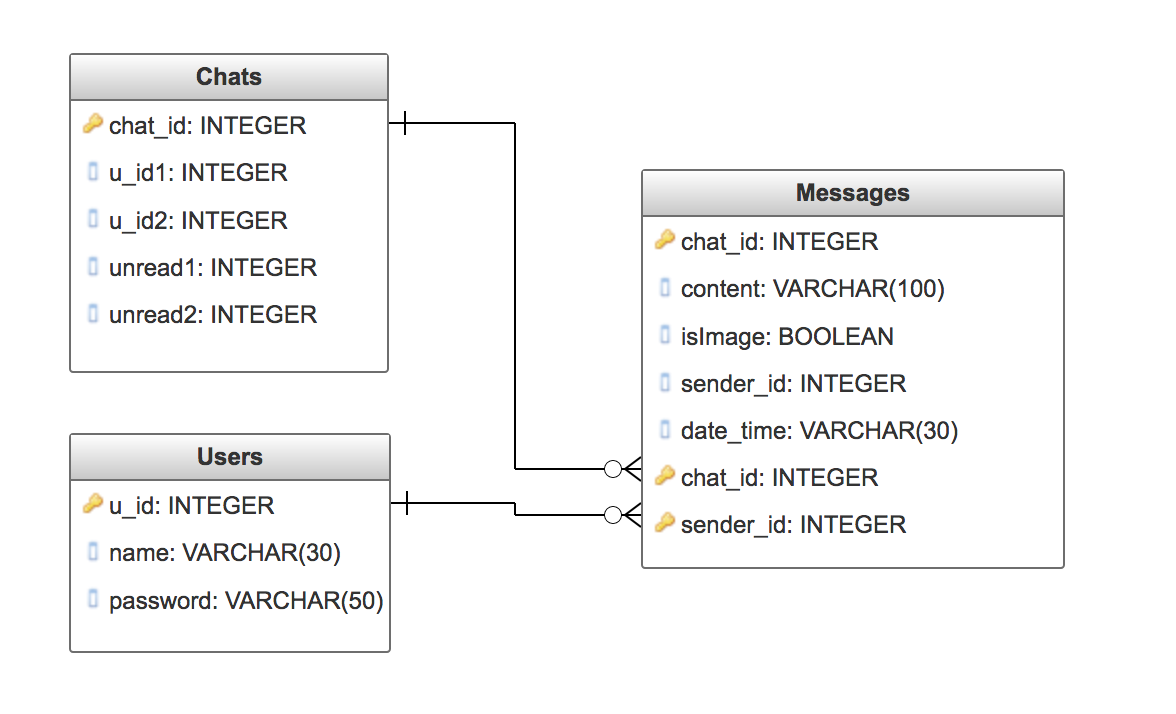
\includegraphics[scale=0.65]{tables.png}
\centering
\end{figure}
\noindent In order to maintain the project's source code, a JavaScript development environment will
need to be present on the host machine (in particular, the React framework). Ensure that the
newest version of the Node.js runtime environment is installed. If not, install Node.js and additional
build tools:
\begin{center} \begin{tabular}{c} \begin{lstlisting}[linewidth=7.5cm]
@$@ sudo apt-get install nodejs
@$@ sudo apt-get install build-essentials
\end{lstlisting} \end{tabular} \end{center}
As of \url{v.8.10} of Node, and \url{v.5.6} of NPM (bundled in the Node installation), a new React
project can be created using:
\begin{center} \begin{tabular}{c} \begin{lstlisting}[linewidth=5.5cm]
@$@ npx create-react-app my-app
@$@ cd my-app
@$@ npm start
\end{lstlisting} \end{tabular} \end{center}
The current project can be run locally from within the \url{messagingSystem} directory by using NPM
to first install missing dependencies (if needed) and start the application:
\begin{center} \begin{tabular}{c} \begin{lstlisting}[linewidth=2.5cm]
@$@ npm install
@$@ npm start
\end{lstlisting} \end{tabular} \end{center}

\end{document}
